% !TeX root = ../main.tex
\section{Link Prediction}
\label{sec:link_prediction}

Die bisherigen Kapitel beschreiben, wer sich trifft. Zum Schluss fragen wir,
ob sich daraus vorhersagen lässt, wer sich künftig trifft. Lassen sich neue
Begegnungen aus der bisherigen Netzwerkstruktur vorhersagen? Und schlägt die
Netzwerkstruktur einfache Faustregeln wie gleiche Nation oder ähnlicher
Jahrgang? Dazu folgen wir dem zeitlichen Experiment von
\textcite{libenNowellKleinberg2007}.

\subsection{Versuchsaufbau}
Wir teilen die Veranstaltungstage in einen Trainingszeitraum von 2016 bis
2019 und einen Testzeitraum von 2021 bis 2025. Das Jahr 2020 lassen wir aus.
Wegen der Corona-Pandemie fanden kaum Wettkämpfe statt. Der Datensatz
enthält für 2020 nur 5\,749 Teilnahmen, in den Jahren davor und danach
jeweils über 13\,000. Zudem trennt die Lücke die beiden Zeiträume klar.

Vorhergesagt wird, welche Athleten künftig am selben Tag eine Bestleistung erzielen. Wir betrachten dabei Athleten, die in beiden Zeiträumen an mindestens drei Veranstaltungstagen erfasst sind. Diese Auswahl ist erst
im Nachhinein möglich, ebenso die Zahl der neuen Kanten, die wir für die
Auswertung verwenden. Eine echte Vorhersage wäre deshalb schwieriger. Das Trainingsnetz enthält alle 7\,024 Athleten des
Trainingszeitraums mit 260\,719 Kanten. Anders als im Arbeitsnetz aus
Kapitel~\ref{sec:reduktion} genügt hier ein gemeinsamer Tag für eine Kante.
Sonst würden Paare, die sich bereits begegnet sind, als neue Kandidaten
gelten. Kandidaten sind alle Paare im Kern, die sich im Training nicht
begegnet sind. Eine neue Kante liegt vor, wenn sich ein solches Paar im
Testzeitraum mindestens einmal trifft (Tabelle~\ref{tab:link_prediction_split}).
Da nur Bestleistungen gespeichert sind und eine Verbesserung den früheren
Tag ersetzt, kann eine neue Kante auch eine frühere, nicht mehr erfasste
Begegnung sein.

\begin{table}[H]
  \centering
  \caption{Datensplit der Hauptanalyse. Trainingskanten zählen Paare
  innerhalb des Kerns, Zufall ist der Anteil neuer Testkanten an allen
  Kandidaten. Eigene Auswertung.}
  \label{tab:link_prediction_split}
  \small
  \begin{tabular}{@{}rrrrr@{}}
    \toprule
    Kernathleten & Trainingskanten & Kandidaten & Neue Testkanten & Zufall \\
    \midrule
    3\,017 & 50\,792 & 4\,498\,844 & 121\,753 & 2,7\,\% \\
    \bottomrule
  \end{tabular}
\end{table}

Wir vergleichen vier Netzwerkverfahren mit drei Faustregeln. Common
Neighbours zählt gemeinsame Nachbarn, Adamic-Adar gewichtet dabei Nachbarn
mit wenigen Kontakten stärker. Preferential Attachment multipliziert nur die
Zahl der Nachbarn beider Athleten. Soundarajan-Hopcroft zählt wie Common
Neighbours und gibt einen Bonus für jeden gemeinsamen Nachbarn, der mit
beiden Athleten in derselben Community liegt. Die Communities bestimmen wir dafür
mit Louvain neu auf dem Trainingsnetz, damit keine Information aus dem
Testzeitraum einfliesst. Die Faustregeln nutzen keine Netzwerkstruktur. Sie
bevorzugen Paare gleicher Nation, ähnlichen Jahrgangs oder zuerst gleicher
Nation und darin ähnlichen Jahrgangs.

Wie bei Liben-Nowell und Kleinberg sortieren wir die Kandidaten nach ihrem
Score und prüfen die ersten $K = 121\,753$ Paare, also so viele, wie
tatsächlich neue Kanten entstehen. Der Anteil richtiger Paare darunter ist
die Precision@K. Geteilt durch die Trefferquote einer zufälligen Auswahl von
2,7\,\% ergibt sich der Faktor gegenüber Zufall. Paare mit gleichem Score
ordnen wir zufällig. Bei zehn verschiedenen Zufallsreihenfolgen ändert sich
die Precision@K um höchstens 0,15 Prozentpunkte.

\subsection{Ergebnisse}
Die Netzwerkverfahren ausser Preferential Attachment treffen fünf- bis
sechsmal so oft wie der Zufall (Abbildung~\ref{fig:link_prediction}). Am
besten ist Soundarajan-Hopcroft mit einer Precision@K von 16,7\,\%. Die
einfache Faustregel gleiche Nation erreicht aber 25,1\,\%, kombiniert mit
dem Jahrgang 25,6\,\%. Die Profilnation stammt allerdings aus dem Jahr 2025.
Hat ein Athlet seither die Nation gewechselt, kann das die Nationsregel
leicht begünstigen. Die Antwort auf
unsere Frage ist damit klar. Die
Netzwerkstruktur sagt neue Begegnungen deutlich besser voraus als der
Zufall, aber schlechter als die Nation allein.

\begin{figure}[H]
  \centering
  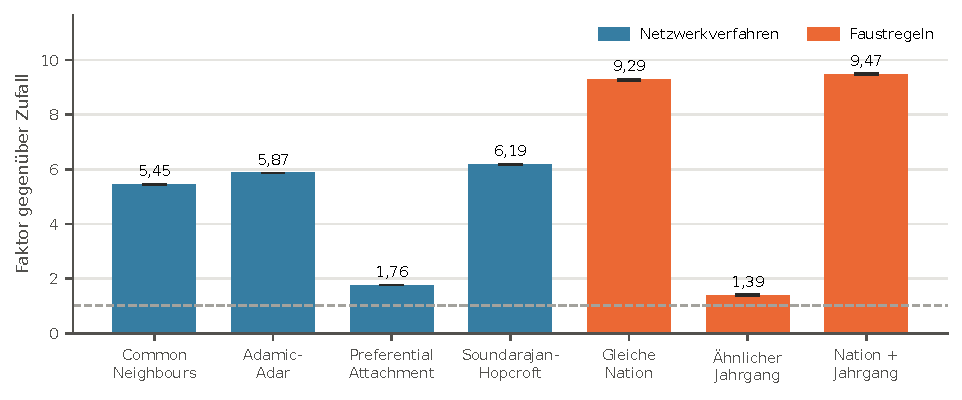
\includegraphics[width=\textwidth]{09_link_prediction.pdf}
  \caption{Faktor gegenüber Zufall je Verfahren im aktiven Kern. Blau
  Netzwerkverfahren, orange Faustregeln, die gestrichelte Linie markiert den
  Zufall (Faktor 1). Die schwarzen Striche zeigen die Spannweite über zehn
  Zufallsreihenfolgen bei gleichen Scores. Eigene Auswertung.}
  \label{fig:link_prediction}
\end{figure}

Fast ein Viertel der neuen Begegnungen (24,0\,\%) findet zwischen
Landsleuten statt, obwohl Landsleute nur 1,2\,\% aller Kandidatenpaare
ausmachen. Von den 55\,986 Kandidatenpaaren aus Landsleuten begegnet sich
mehr als die Hälfte (52,2\,\%) im Testzeitraum, über alle Kandidaten sind es
2,7\,\%. Nationale Meisterschaften wiederholen sich jedes Jahr und bringen
Landsleute, die sich bisher nicht begegnet sind, häufig zusammen. Das passt zu den wiederholten Begegnungen aus
Kapitel~\ref{sec:zusammenhalt} und zur nationalen Assortativität aus
Kapitel~\ref{sec:assortativitaet}. Die Netzwerkverfahren erkennen dieses
Muster nur teilweise. Unter den besten Paaren von Common Neighbours,
Adamic-Adar und Soundarajan-Hopcroft verbinden 17 bis 20\,\% Landsleute.
Vermutlich prägen die internationalen Veranstaltungen, die nach
Kapitel~\ref{sec:zusammenhalt} das Netz zusammenhalten, auch die
gemeinsamen Nachbarn. Auch die
Communities im Trainingsnetz sind gemischt, im Mittel stellt die grösste
Nation nur 34\,\% ihrer Mitglieder. Der Community-Bonus hebt die Precision@K
gegenüber Common Neighbours dennoch von 14,8 auf 16,7\,\%.

Preferential Attachment erreicht nur 4,8\,\%. Viele Kontakte entstehen durch
wenige grosse Meisterschaften (Kapitel~\ref{sec:zentralitaet}), daraus folgt
nicht, wen ein Athlet als Nächstes trifft. Überraschend schwach ist auch die
Faustregel Jahrgang mit 3,8\,\%, obwohl der Jahrgang in
Kapitel~\ref{sec:assortativitaet} das stärkste Merkmal war. Gleichaltrige
Paare gibt es aber sehr viele. Von den 340\,638 gleich alten
Kandidatenpaaren begegnen sich nur 3,8\,\% im Testzeitraum, kaum mehr als
über alle Kandidaten.
Eine hohe Assortativität bedeutet also nicht, dass sich ein Merkmal gut zur
Vorhersage eignet.

Abbildung~\ref{fig:link_prediction_robustheit} zeigt zwei
Robustheitsprüfungen. Verlangen wir für eine neue Kante mindestens zwei
gemeinsame Testtage, bleiben 32\,636 neue Kanten, und die Nationsregeln
liegen noch deutlicher vorne. Wiederholte neue Begegnungen sind also noch
stärker national. Bestimmen wir den Kern nur über den Trainingszeitraum,
umfasst er 5\,594 Athleten. Darunter sind auch Athleten, die später nicht
mehr erfasst sind. Die Trefferquote des Zufalls sinkt deshalb von 2,7 auf
0,8\,\%, und mit ihr die Precision@K aller Verfahren. In beiden
Prüfungen bleiben die Nationsregeln klar vorne, gefolgt von
Soundarajan-Hopcroft.

\begin{figure}[H]
  \centering
  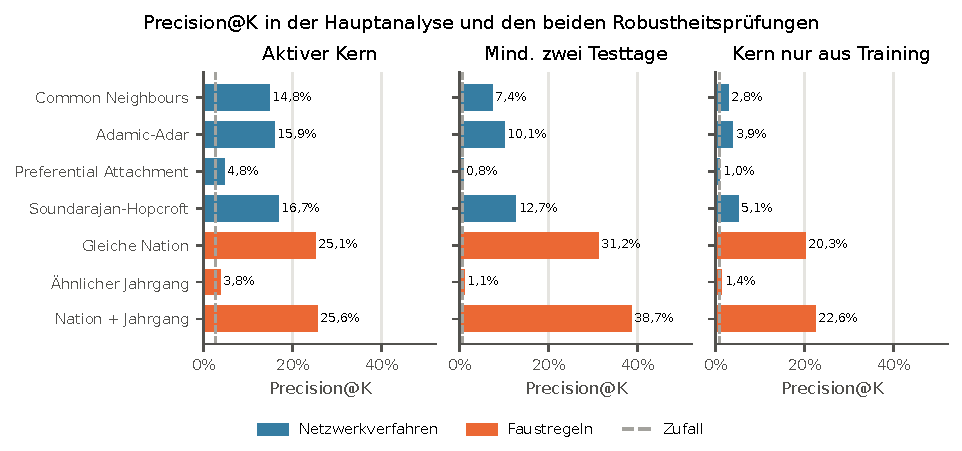
\includegraphics[width=\textwidth]{09_precision_robustheit.pdf}
  \caption{Precision@K je Verfahren im aktiven Kern, bei mindestens zwei
  gemeinsamen Testtagen und bei einem nur über das Training bestimmten
  Kern. Blau Netzwerkverfahren, orange Faustregeln, die gestrichelte Linie
  zeigt die Trefferquote einer zufälligen Auswahl im jeweiligen Szenario.
  Eigene Auswertung.}
  \label{fig:link_prediction_robustheit}
\end{figure}
